\documentclass[11pt, spanish, a4paper, twoside]{article}

% Versión 1.er cuat 2021 Víctor Bettachini < vbettachini@unlam.edu.ar >

\usepackage[T1]{fontenc}
\usepackage[utf8]{inputenc}

\usepackage[spanish, es-tabla]{babel}
\def\spanishoptions{argentina} % Was macht dass?
% \usepackage{babelbib}
% \selectbiblanguage{spanish}
% \addto\shorthandsspanish{\spanishdeactivate{~<>}}

\usepackage{graphicx}
\graphicspath{{./figuras/}{../LaTeX/}}
% \usepackage{float}

\usepackage[arrowdel]{physics}
\newcommand{\pvec}[1]{\vec{#1}\mkern2mu\vphantom{#1}}
% \usepackage{units}
\usepackage[separate-uncertainty= true, multi-part-units= single, range-units= single, range-phrase= {~a~}, locale= FR]{siunitx}
\usepackage{isotope} % $\isotope[A][Z]{X}\to\isotope[A-4][Z-2]{Y}+\isotope[4][2]{\alpha}

\usepackage{tasks}
\usepackage[inline]{enumitem}
% \usepackage{enumerate}

\usepackage{hyperref}

% \usepackage{amsmath}
% \usepackage{amstext}
% \usepackage{amssymb}

\usepackage{tikz}
\usepackage{tikz-dimline}
\usetikzlibrary{calc}
% \usetikzlibrary{math}
\usetikzlibrary{arrows.meta}
\usetikzlibrary{snakes}
\usetikzlibrary{decorations}
\usetikzlibrary{decorations.pathmorphing}
\usetikzlibrary{patterns}

\usepackage[hmargin=1cm,vmargin=3cm, top= 0.75cm,nohead]{geometry}

\usepackage{lastpage}
\usepackage{fancyhdr}
\pagestyle{fancyplain}
\fancyhf{}
\setlength\headheight{28.7pt} 
\fancyhead[LE, LO]{\textbf{Mecánica General} }
\fancyhead[RE, RO]{\href{https://ingenieria.unlam.edu.ar/}{$\vcenter{\hbox{
\includegraphics[height=1cm]{ambos.pdf}}}$}}
\fancyfoot{\href{https://creativecommons.org/licenses/by-nc-sa/4.0/deed.es_ES}{$\vcenter{\hbox{
\includegraphics[height=0.4cm]{by-nc-sa_80x15.pdf}}}$} \href{https://ingenieria.unlam.edu.ar/}{DIIT - UNLaM}}
\fancyfoot[C]{ {\tiny Actualizado al \today} }
\fancyfoot[RO, LE]{Pág. \thepage/\pageref{LastPage}}
\renewcommand{\headrulewidth}{0pt}
\renewcommand{\footrulewidth}{0pt}


\begin{document}
\begin{center}
  % \textsc{\large Mecánica general}\\
  \textsc{\large Fuerzas de ligadura | Multiplicadores de Lagrange} 
\end{center}

\begin{enumerate}


	
\item 
\begin{minipage}[t][1.1cm]{0.75\textwidth}
\textbf{Péndulo rígido ideal}\\
Calcule la tensión de la cuerda con el método de multiplicadores de Lagrange.
La restricción es que la pesa se mantiene siempre en \(\vec{r} = \ell \hat{\rho}\), ergo la función que expresa esto es \(f(\rho) = \rho - \ell = 0\).
\end{minipage}
\begin{minipage}[c][0cm][t]{0.25\textwidth}
	\begin{tikzpicture}[scale= 1.0]
  	\draw [arrows=-latex] (-1,2) -> (-1,1) node [above=15, right=2] {\(\vec{g}\)}; % g vertical
		\draw [ultra thick] (-1.5,3) -- (2,3);
		\fill [pattern = north east lines] (-1.5,3) rectangle (2,3.2); % techo
		\draw [dashed] (0,3) -- (0,-.25);	% vertical
		\draw [thick] (0,3) -- +(-60:3) node[midway,above,right=2] {\(\ell\)};	% inclinada +:relativa, -60 grados, longitud 3
		\shade [ball color=black!80] ($(0,3)+(-60:3)$) circle(0.25) node [] {\color{white} $m$};
    \draw [arrows=-latex] (0,.4) -> (1.25,.4) node [midway, above] {\( \psi \)}; % desplazamiento horizontal
		\draw [arrows=-latex] (0,0) arc [start angle=-90, end angle=-65, radius=3] node [below=12, left=8] {\( \varphi \)};
	\end{tikzpicture}
\end{minipage}



\item 
\begin{minipage}[t][4cm]{0.42\textwidth}
\textbf{Cilindro que rueda por un plano inclinado} [Marion (e) ex. 7.5]\\
% English \textbf{Marion ejemplo 6.5 y ejemplo 7.9} Disco rodando en un plano inclinado.
	\begin{enumerate}
		\item Encuentre las ecuaciones de movimiento, 
		\item la aceleración angular,
		\item y la fuerzas de ligadura. 
	\end{enumerate}
\end{minipage}
\begin{minipage}[c][2.5cm][t]{0.3\textwidth}
	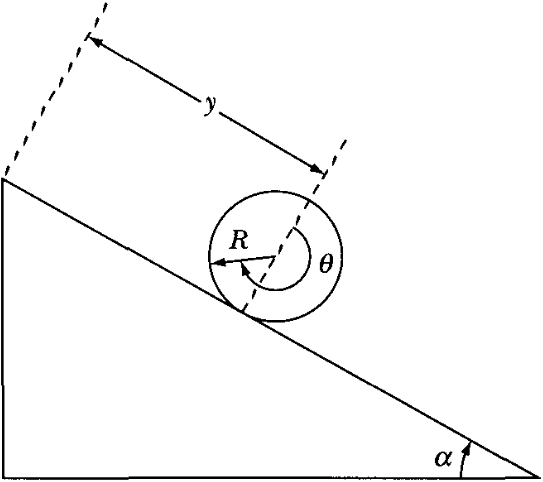
\includegraphics[width=\textwidth]{marion_fig6_7}
\end{minipage}


	
\item
\begin{minipage}[t][8.5cm]{0.55\textwidth}
\textbf{Doble máquina de Atwood}

[Marion (e) ex. 7.8 y ejercicio 7-37]\\
Utilice el sistema de coordenadas indicadas.
Para este sistema de poleas determine: 
\begin{enumerate}
	\item las ecuaciones de movimiento,
	\item y las tensiones de ambas cuerdas utilizando el método de multiplicadores de Lagrange.
\end{enumerate}
\end{minipage}
\begin{minipage}[c][0.5cm][t]{0.4\textwidth}
	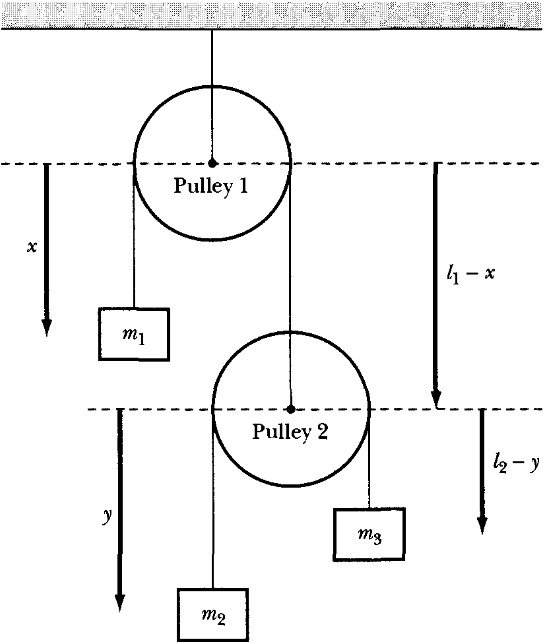
\includegraphics[width=\textwidth]{marion_fig7_6}
\end{minipage}



\item 
\textbf{Pesos enlazados por una cuerda} [Taylor 7.50]\\
Una pesa de de masa \(m_1\) está posada sobre una mesa horizontal.
Está atada a una cuerda dispuesta horizontalmente hasta una pequeña polea (masa despreciable) que no ofrece fricción en el borde de la mesa.
En el otro extremo de la cuerda cuelga otra pesa de masa \(m_2\).

Llame las distancias a \(m_1\) y \(m_2\) desde la polea \(x\) e \(y\) respectivamente.
Estas satisfacen la ecuación de restricción \(f (x, y) = x + y -l = 0\), siendo \(l\) la longitud de la cuerda.
\begin{enumerate}
\item Escriba las dos ecuaciones de Lagrange modificadas y resuélvalas (juntos con la ecuación de restricción) para \(x, y\) y para el multiplicador de Lagrange \(\lambda\).
\item Encuentre las fuerzas de tensión sobre ambas masas.
\item Verifique sus respuestas resolviendo el problema con la metodología Newtoniana.
\end{enumerate}




\item 
\begin{minipage}[t][3cm]{0.62\textwidth}
\textbf{Partícula deslizando sobre una semi-esfera} [Marion (e) ex. 7.10]\\ 
La partícula de masa \(m\), considerada puntual, desliza sobre una semi-esfera de radio \(R\) sin fricción.
Encuentre: 
\begin{enumerate}
	\item la fuerza de la ligadura, 
	\item y el ángulo en que la partícula se despega de la semi-esfera.
\end{enumerate}
\end{minipage}
\begin{minipage}[c][0cm][t]{0.3\textwidth}
	% \includegraphics[width=\textwidth]{marion7_10}
	\begin{tikzpicture}[scale= 1.0]
		\draw [ultra thick] (-3,0) -- (3,0);
		% \draw [ultra thick] (-3,0) -- (3,0);
		\fill [pattern = north east lines] (-3,0) rectangle (3,-0.2); % piso
		\draw [ultra thick] (-2,0) .. controls (-2,2*0.555) and (-2*0.555,2) .. (0,2) .. controls (2*0.555,2) and (2,2*0.555) .. (2,0); % semi esfera
		% \filldraw (0,2.2) circle (0.2); % masa superior
		% \fill (2*0.5+.12,1.732+.18) circle [radius=0.25] node [midway, text=white] { \( m \) };
		% \filldraw (2*0.5+.12,1.732+.18) circle (0.2) node [above, right=5] {\(m\)}; % masa a la derecha
		\shade [ball color=black!80] (2*0.5+.12,1.732+.18) circle(0.2) node [] {\color{white} $m$};
		% \draw (2,2) circle [radius=0.3, color=white, fill=black] node {$T_1$};
		\draw [dashed] (0,0) -- (0,2); % linea vertical
		\draw [-LaTeX] (0,0) -- (1,1.732) node [midway, anchor=west] {\(R\)}; % linea hacia la derecha
		\draw [-stealth] (0,1) arc (90:60:1) node [above left] {\(\theta\)}; % arco c/ flecha comenzando en (0,1), de 90 a 60 grados, 1...
		% \node [circle,draw,label=60:$60^\circ$,label=below:$-90^\circ$] {\(m\)}; 
		% \node at (-2*0.5+.15,1.732+.15) [circle,draw,fill=black] {\(m\)}; 
		\draw [-stealth, thick] (-2.5,2) -> (-2.5,1) node [above=15, right=2] {\(\vec{g}\)}; % g vertical
	\end{tikzpicture}
\end{minipage}



\end{enumerate}
\end{document}
